%% introduction.tex
%%

%% ==============================
\chapter{Einleitung}
\label{ch:Introduction}
%% ==============================
"Ein Mensch lernt sein Leben lang." \par

Dieser weise Spruch ist allgemein gültig. Jeder Mensch, sei es im Beruf oder im privaten Umfeld muss neue Inhalte erlernen. Wie schnell er dies tut, das hängt von seinem individuellem Lerntempo ab. Damit er eine Lernhilfe erhält und neue Inhalte interessant aufbereitet, gibt es computerbasierte Hilfesysteme. Diese Hilfesysteme sind dafür da, um neue Inhalte schnell zu lernen. Wie ein solches Hilfesystem aussehen kann wird in dieser Arbeit vorgestellt. Die neuen Lerninhalte beziehen sich auf eine spezielle Software, welche bei der Ausschreibung des Seminarthemas vorgeschrieben wurde. Diese Software soll im Folgenden kurz erläutert werden.




\section{CAS Campus}
Die Zielsoftware, worauf unsere spätere Empfehlung basiert, ist die Software CAS Campus. Diese Software ist von der CAS Software AG aus Karlsruhe. Das Ziel der Software ist es einen kompletten Student-Lifecycle (siehe Abbildung \ref{img1:stdLife}) nachzubilden. Der Lifecycle beginnt mit der Bewerbung des Studenten an einer Hochschule und endet mit dem Alumni Zustand\footnote{Quelle: http://cas-education.de entnommen am 27.07.15}. Bevor ein Student zu dem Alumni-Zustand kommt, muss er zuvor einige Stationen begleiten. Die Software CAS Campus soll den Studenten genau auf diesem Weg begleiten, indem alle Prozesse abgebildet werden. Die Prozesse sind hierbei sehr vielschichtig. Sie reichen vom einfachen Eintragen der Noten bis hin zu einer komplexen Modellierung von ganzen Studiengängen. Weitere Prozesse sind beispielsweise Terminmanagement. Hier müssen Vorlesungen zu Räumen zugeordnet werden und auf Konflikte bei der Belegung geprüft werden. Im Mittelpunkt dieser Prozesse steht immer der Student. Er ist sozusagen der Endkunde der Anwendung und steht im Zentrum eines modernen Campus-Management-Systems.\par



\begin{figure}[ht]
\begin{center}
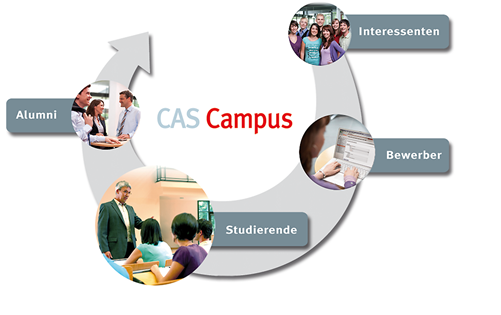
\includegraphics[width = 0.5\textwidth]{casCampus.png}
\caption{Student-Lifecycle}
\label{img1:stdLife}
\end{center}
\end{figure} 

\section{Motivation}
Das Ziel dieser Arbeit ist es, eine mögliche Lösung zu finden, wie eine adaptive Online-Lernhilfe aussehen kann. Hierzu müssen passende Lösungsansätze gefunden werden. Die Lösungsansätze müssen auf die Zielsoftware CAS Campus angewandt werden können, so dass eine spätere Implementierung der Lösung erfolgen kann.  Wichtig hierbei ist die Zentrierung auf den Nutzer. Diese Zentrierung wurde als Vorgabe zur Adaptivität der Lösung Vorgegeben und soll sich in allen Lösungsansätzen widerspiegeln.  

\section{Weiteres Vorgehen}
Im folgenden Text wird zuerst der aktuelle Status-Quo in Sachen Lernen und Online-Hilfe erläutert. Darauf aufbauend wird erklärt, was genau Adaptiv für unsere Arbeit bedeutet und worauf wir unseren Schwerpunkt beziehen. Zur besseren Einführung in die Thematik werden die Nutzer und deren Probleme in Form von Personas vorgestellt. Diese Nutzer werden anschließend Klassifiziert, damit bessere Lösungsansätze gefunden werden können. Anhand der Klassifizierung werden wir unsere Lösungsansätze vorstellen, diese kritisch bewerten und eine anschließende Empfehlung daraus generieren. Zum Abschluss der Arbeit möchten wir ein kleines Fazit mit Ausblick auf ein weiteres Vorgehen bei der Arbeit geben.


